\documentclass[11pt]{sig-alternate}
\usepackage{hyperref}
\usepackage{tabularx}
\usepackage{graphicx}
\usepackage{blindtext}
\usepackage[utf8]{inputenc}
\usepackage[english]{babel}
\usepackage{lastpage}
\usepackage{comment}
\usepackage{dirtytalk}
\usepackage{xcolor}
\usepackage{hanging}
\usepackage{wrapfig}
\usepackage[backend=biber, style=apa]{biblatex}
\addbibresource{notation.bib}
\usepackage{authblk}
\usepackage{caption}
\usepackage{subcaption}
\usepackage{graphicx,subfigure}
\usepackage{authblk}

\usepackage{fancyhdr}
\pagestyle{fancy}
\renewcommand{\headrulewidth}{0pt}
\renewcommand{\footrulewidth}{0pt}
\setlength\headheight{80.0pt}
\addtolength{\textheight}{-80.0pt}
\chead{%
  \ifcase\value{page}
  % empty test for page = 0
  \or 
\includegraphics[width=\textwidth]{headerImage.png}% page=1
  \or 
\includegraphics[width=\textwidth]{headerImage.png}% page = 2
  \or 
\includegraphics[width=\textwidth]{headerImage.png}% page = 3
  \or 
\includegraphics[width=\textwidth]{headerImage.png}% page = 4
  \or 
\includegraphics[width=\textwidth]{headerImage.png}% page = 5
  \else
  
\includegraphics[width=\textwidth]{headerImage.png}
  \fi
}
%\chead{
\includegraphics[width=\textwidth]{headerImage.png}}
\fancyfoot[LE,LO]{Out-of-school STEM Program for Students with Visual Impairments: Adaptations and Outcomes During the COVID-19 Pandemic\\           
DOI: 10.14448/jsesd.13.0004}
\fancyfoot[CE,CO]{{ }}
\fancyfoot[RE,RO]{\thepage}
\pagenumbering{arabic}
\hypersetup{
    colorlinks=true,
    urlcolor=blue
}
 
\let\oldabstract\abstract
\let\oldendabstract\endabstract
\makeatletter
\renewenvironment{abstract}
{\renewenvironment{quotation}%
               {\list{}{\addtolength{\leftmargin}{1em} % change this value to add or remove length to the the default
                        \listparindent 1.5em%
                        \itemindent    \listparindent%
                        \rightmargin   \leftmargin%
                        \parsep        \z@ \@plus\p@}%
                \item\relax}%
               {\endlist}%
\oldabstract}
{\oldendabstract}
\makeatother

% Left align captions
\captionsetup{justification   = raggedright,
              singlelinecheck = false}
              
\begin{document}


\title{Out-of-school STEM Program for Students with Visual Impairments: Adaptations and Outcomes During the COVID-19 Pandemic}

\author[1]{\large \color{blue}Sunggye Hong}
\author[1]{\large \color{blue}Irene L. Topor}
\author[1]{\large \color{blue}Jinseok Park}
\author[1]{\large \color{blue}Tasnim A. Alshuli}

\affil[1]{University of Arizona}

\toappear{}

\maketitle
\begin{@twocolumnfalse} 

\begin{abstract}
     \textit{Although previous research exists on making adaptations for students with Visual Impairments (VI) in online settings, there is limited research on the teaching and learning dynamics of students with VI during the COVID-19 pandemic. Since responses to the pandemic made it difficult for students with VI to participate in educational opportunities that require hands-on experiences, gaps have been identified in gaining access to educational opportunities. Project POEM, a STEM project-based intervention for students with VI, was originally planned with programs based on in-person modes, aimed at increasing motivation and awareness of science, technology, engineering, and math of students with VI. Due to limitations of in-person participation, substantial modifications and adaptations were required for the programs to be meaningful and effective when delivered in online environments. It was found that proficiency in the use of technology options, specific instruction and guidance for access of information, and program planning in advance were the three key elements for successful implementation of the programs. This article documents 1) existing research on the impacts of the pandemic, 2) meaningful adaptations and modifications, 3) essential elements for developing online programs in STEM, and 4) identified strategies in program transition for students with VI. Some skills may not be most efficiently taught through online interactions, however participation of family members, careful modifications of existing activities, and sufficient level of technology support allows many skills to be acquired through online learning. Most importantly, strong collaboration of participating team members makes it possible for students with VI to participate equitably in online environments.}
     \\\\
     \textbf{Keywords:} Students with Visual Impairments, STEM, COVID-19, Online learning
\end{abstract}
\end{@twocolumnfalse}

%% ABSTRACT


%% AUTHOR INFORMATION
\\ \\ \\
\textbf{*Corresponding Author, Sunggye Hong} \href{mailto:sghong@arizona.edu}{(sghong@arizona.edu)} \\
\textit{Submitted May 5, 2022 }\\
\textit{Accepted December 5, 2022} \\
\textit{Published online April 15, 2023} \\
\textit{DOI: 10.14448/jsesd.14.0003} \\


\pagebreak
\pagebreak

\vspace{5mm}
\section*{\vspace{140mm}}
\section*{Introduction}
\begin{large}

From Spring 2020, the COVID-19 pandemic unexpectedly forced people to make rapid transitions in education. All K-12 to higher education programs closed or transitioned to online learning. The sudden change was more challenging to students with Visual Impairments (VI), including blindness and low vision, because preventive and mitigative strategies of the pandemic made it difficult for students with VI to participate in educational opportunities requiring fewer physical interactions. The change to online learning led to limited access to learning engagement for students with VI that formerly was accessible by touching or approaching an object closer to see. 

Compared to students without disabilities, students with VI have additional difficulties mainly because textbooks, materials, and educational activities often require accompanying hands-on experiences. Combined with students' lack of instructional times between extended core curriculum and general curricula activities, such gaps are much more severe (Hamid, 2020). These difficulties resulted in 13 percent of students with VI not receiving special education service and 43 percent of them experienced a lack of support to access online learning during the pandemic (Rosenblum et al., 2020).

With the pandemic shutdown forcing school closings, professionals who serve students with VI did not have sufficient time to prepare for the rapid transition to service delivery, the way specialized educational services were changed for students with VI. Rosenblum and her colleagues (2020) investigated the impacts of the pandemic by surveying 1,208 professionals who serve students with VI, including teachers of students with VI and orientation and mobility specialists. The researchers found that the professionals could not use school facilities to create learning materials and struggled with forced transitions to online platforms for instructions. Challenges existed when providing hands-on learning materials not available at home. Another challenge was increased difficulty in collaboration between teachers, families, and professionals who work with students with VI. Parents commented that classroom teachers did not fully understand the needs of students to engage in online learning. The transition caused limited opportunities for professionals for VI to work together to provide adequate accommodations for students with VI (Smith, 2020).

During the pandemic, lack of technology readiness of students with VI significantly affected learning engagement in virtual settings. Because in-person options were not allowed, increased dependency on technology was challenging to students with VI when engaged in online learning settings. McBride (2020) conducted a survey and found that students with VI did not have sufficient time to learn essential technology skills associated with online learning, including screen readers and magnifiers, virtual meeting software, and computer use in general during this unexpected transition. The challenges varied depending on students’ previous training experience and familiarity with specific technology options. Also, inaccessible websites and software added an additional layer of challenges for students with VI (Mulliken, 2017), which resulted in limited engagement in the virtual classes. 

Despite these challenges, transition to virtual settings provided opportunities to expand existing in-person educational programs to both in-person and online learning environments for students with VI. Established collaborations during the pandemic enabled instructors to adapt learning activities based on adapting visual needs in remote settings. For instance, Lepore-Stevens et al. (2021) and Foster et al. (2020) reported exemplary adaptations experiences in developing online physical activity programs using videoconferencing and online communication tools. Pre-recorded videos live sessions using verbal description and auditory coaching allowed successful continuation of the programs with high engagement rates of the participants with VI.

While there have been studies conducted to determine the overall impacts of the pandemic on students with VI, limited information could be found for ways that after-school programs could better accommodate students with VI during this transition, a gap that our work might help to resolve. Lack of specific ideas and procedures for collaboration for setting up and administering extra-curricular activities may provide more significant insights for professionals who plan to implement programs in Science, Technology, Engineering, and Math (STEM). The purpose of this paper is to present how our team adapted our out-of-school STEM program for students with VI amid the pandemic. When considering that all sectors in education were disrupted, it is understandable that few educational programs have described pandemic adaptation strategies, and with limited literature focused on transition, literature focusing on transition experiences with students with VI could fill the gap. Project POEM originally included realistic and hands-on science and engineering learning experiences in in-person and online settings. After the pandemic outbreak, we attempted significant adaptations to mitigate the situation and continue our program implementation. This paper will present adaptation strategies utilized in technology use and communication between students and mentors in our out-of-school STEM learning program. Our curriculum adaptation will provide insightful strategies for planning and implementing online STEM programs for students with VI.

\section*{Project POEM Overview}

Project POEM (Project-Based Learning Opportunities and Exploration of Mentorship for Students with VI in STEM) attempted to raise awareness and motivation towards STEM careers among students with VI, using the Project-Based Learning (PBL) framework based on Next Generation Science Standards (NGSS) and hands-on STEM experiences (NGSS Lead States, 2013). The NGSS combines scientific practice scientists use to investigate the natural world and engineers use to build engineering models and systems including: 1) asking questions and defining problems, 2) developing and using models, 3) planning and carrying out investigations, 4) analyzing and interpreting data, 5) using mathematical and computational thinking, 6) constructing explanations and designing solutions, 7) gathering, evaluating, and communicating information. For example, the project used an engineering practice for making the Reconnaissance Orbiters and allowed the participants to create a whole object using parts (NGSS’s MS-ETS1-1 and MS-ETS1-2). Students are expected to ask and answer inquiry-based questions leading to descriptions and explanations of phenomena and empirical pieces of evidence. The POEM’s practice also aims to help students generalize ‘scientific inquiry’ and ‘engineering design’ from STEM learning to everyday life [See Kortenkamp et al. (2021) and Lunsford et al. (in press) to learn more about Project POEM].

Dr. Sukhai, a scientist who has a VI, noted in his April 20, 2015 blog posting that "[There is a] lack of mentors/role models in the field; inaccessible laboratories; lack of access to assistive technologies and alternative formats; negative attitudes of educators and service providers; a knowledge gap on how to instruct a student with a disability; and, a lack of knowledge of how to solve logistical concerns around integrating students with disabilities in STEM fields." Inviting students with VI into STEM fields and raising their awareness of the subject areas goes beyond simple adaptations and delivery of assistive technology equipment. Project POEM aimed to reduce the observed gaps using the original curriculum developed by its project team with diverse backgrounds (e.g., science instructors, educators of students with VI, experienced teachers in online learning, and technology experts). The primary goal that the project addressed is to understand better how the combination of PBL and mentoring can provide middle and high school (grades 7-11) students with VI experiences necessary to pursue STEM subjects and careers. PBL-based teaching aims to engage students in an inquiry-driven process with hands-on activities and replace traditional STEM-learning into increased discussion, mentoring, advising, and creating final learning outcomes. Students’ interests and motivations of learners become the primary focus in PBL learning (Tal et al., 2006). The project, taught first in person, developed, and implemented three major activities to achieve these goals, described below. 

\section*{\textit{Readiness Academy}}

The Readiness Academy was designed to acquaint students with VI with STEM based PBL through hands-on activities. In the summers of 2018 and 2019, students with VI were invited to Tucson, Arizona, for approximately a week to participate in the Readiness Academy. The University of Arizona (UA) in Tucson has a facility operated by the Department of Astronomy on Mt. Lemmon, about 50 miles away from the main campus. Sky School traditionally works with local school districts to encourage high school student participation in Sky School throughout the regular school year to learn about being a scientist and the scientific process. Project POEM sought to provide similar activities and access to STEM and the process of science for students with VI. The Project POEM students stayed in the Sky School dormitory and participated in the daily activities designed to immerse them into the components of PBL, including working with the science and engineering practices and disciplinary core ideas of the NGSS (2013) of developing hypotheses, collecting data based on the hypotheses that they have developed, analyzing collected data, and finally presenting and communicating their findings with others. POEM students were provided with descriptions and a guided tour of the Sky School. The students had a moderated conversation with staff members and came up with an hypothesis: how different types of tree species would affect soil and lake water content”. They devoted the next several days to testing this hypothesis, collecting soil samples, analyzing collected data, and creating a presentation.

Sky School scientists served as the primary instructors for introducing various scientific concepts. These scientists majored in STEM fields and worked previously in Sky School, providing similar instructions for sighted students. POEM students were exposed to the Sky Island Adventure’s ecology, biology, geology, and astronomy. The project utilized expertise of Sky School scientists since they all majored in science-related areas. For example, dendrochronology (study of tree rings), wildlife, atmosphere (climate change) were expertise areas of these scientists. We also invited other faculty members who could provide additional insights about these scientific areas of inquiry. Project POEM senior personnel worked closely with the Sky School scientists to adapt and ensure all activities and materials were accessible to students with VI during its first two rounds, where students with VI were all invited to in-person activities at the Sky School site located in Tucson. Throughout the Readiness Academy, master’s students preparing to be certified Teachers of students with Visual Impairments (TVI) participated as assistants so they could build their own skills and learn how to adapt STEM activities for students with VI.

For the first two years of POEM, students with VI arrived at the Sky School on Sunday afternoon and were provided with an overview of the facility as well as programs for the next several days. Students with VI were then engaged in a series of science activities and presentations provided by the Sky School scientists and worked collaboratively with preservice TVI candidates. To run the program effectively, students were divided into two small groups. Each group was asked to develop an original hypothesis that they would work on the next several days during their participation in the Sky School activities. The list of adaptations and assistive technology devices provided to students with VI included braille, large print, and accessible computers with JAWS (Job Access with Speech), a screen reading software, and ZoomText, and a screen magnifying software. Students were encouraged to use various types of assistive technology devices during the activity’s data collection and data analysis phases. These tactile aids and technology could be implemented reasonably well because students and scientists were all present in Tucson and project team members could make fine adjustments as needed during the week-long activity. Four preservice candidates in 2018 and three in 2019 participated during the Sky School, serving as the liaisons between the science instructors and students. Both the scientists and the preservice TVI candidates participated in four hours of prerequisite training which covered topics such as best instructional methods for working with students with vi, examples of hands-on strategies, common scenarios of science lessons for students with VI, and basic orientation and mobility techniques. We included two presentations where the value of accessible laboratory environment for people with VI using accessible data analysis methods as well as appropriate tools such as Talking Lab-quest, a set of a tablet computer and specially designed sensors could be discussed. Lodging, meals, transportation, and equipment during the Readiness Academy were all provided free of charge to participants.

\section*{\textit{Exploration Activities}}

Once the Readiness Academy was completed, students returned home and participated remotely in more science-led activities. During this phase of the project, students were engaged in two primary objectives. They were to understand the accommodations and adaptations required for working as scientists with VI and to further their practice in PBL. Both activities utilized mentoring as the primary facilitation vehicle. The POEM mentor training was adapted from the Entering Mentoring curriculum, which was developed to prepare mentors of undergraduate researchers through eight, weekly discussion seminars on: getting started, communication, goals, identifying challenges, resolving challenges, evaluating progress, elements of good mentoring, and developing a mentoring philosophy (Balster, Pfund, Rediske, \& Branchaw, 2010; Handelsman, Pfund, Lauffer \& Pri-\\bbenow, 2005). We adapted the content to eight modules and all mentors took part in the training. Additional training module for working with people who are blind or visually impaired were added for university mentors who did not have previous background in working with this population.

Mentor recruitment was conducted through outreach and collaborative efforts. Points (a) – (c) pertain to recruitment of mentors in STEM fields where as (d) – (f) pertain to recruitment of mentors with VI (industry) as follows: a) information posted on the project's website; (b) postings on listservs, websites, and/or in newsletters of consumer organizations; (c) contacting undergraduate students in STEM majors; (d) contacting member of the National Federation for the Blind computer and science division; (e) contacts of the project team members (f) extensive research on Facebook.

First, mentors with VI helped students with VI to complete monthly assignments associated with understanding the demands for working as scientists with VI. Mentors with VI should be currently working in STEM fields. List of assignments included an interview with the mentor to learn about their VI; training for their job and accommodations used on the job site; virtual observation of the mentor working on the job site; keeping an assistive technology log of apps, programs, and technology both the mentor and student use over a weeklong period and comparing them; and having the student interview both the mentor and a co-worker without VI to ascertain similarities and differences in how each does the job.

Simultaneously, students with VI were matched with a university mentor majoring in STEM fields to further their experiences in STEM learning through PBL. The project team devised an original curriculum utilizing monthly activities that included Three-Dimensional (3D) printing objects (e.g., topographic terrains of craters, asteroids, and Mars/Moon) and Two-Dimensional (2D) tactile graphics (e.g., robotic spacecraft modules). The project curriculum based on NGSS (2013) included monthly assignments for students with VI. Each student worked with their university mentors to complete their assignments and submit their outcomes or results to the project team. For example, by comparing Mars to Earth, students with VI would better understand geologic processes and how they affected a planet over time.

Dr. Kortenkamp, the project's co-principal investigator, identified several geologic characteristics that the planet Mars has in common with the Arizona region. These areas are asteroid impact craters, canyon systems, and sand dunes. The impact crater module includes the study of the Meteor Crater near Flagstaff, AZ. This pristine asteroid impact crater is the most comprehensively studied crater in the solar system, which assisted students with VI in expanding their studies to explore impact craters on Mars, with particular emphasis on the evidence for liquid water inside the Martian craters. Finally, the relative proximity of Imperial Sand Dunes National Recreation Area near the Arizona/California/Mexico border serves as the ju-\\mping-off point to explore the vast diversity of sand dunes on Mars. The prompts included in each month for students with VI consist of inquiry-based questioning entitled “List of Wonders,” data gathering and recording, and presentation to answer the inquiries using STEM-related communication skills. This format was intentionally designed for practicing their skills using the PBL process. These activities were completed remotely using email, Facetime, messaging, and other social network services.

\section*{\textit{Enrichment Institute}}

Once students with VI completed their Exploration Activities, they returned to the University of Arizona campus in Tucson, Arizona for a week. The purpose of this final activity was to experience university life as a student with VI including daily living, STEM learning, orientation and mobility skills, and other skills necessary to participate in a university curriculum. During the day, students with VI visited labs and job sites in STEM-related fields. 
{\begin{figure}[htp] 
    \leftmargin
    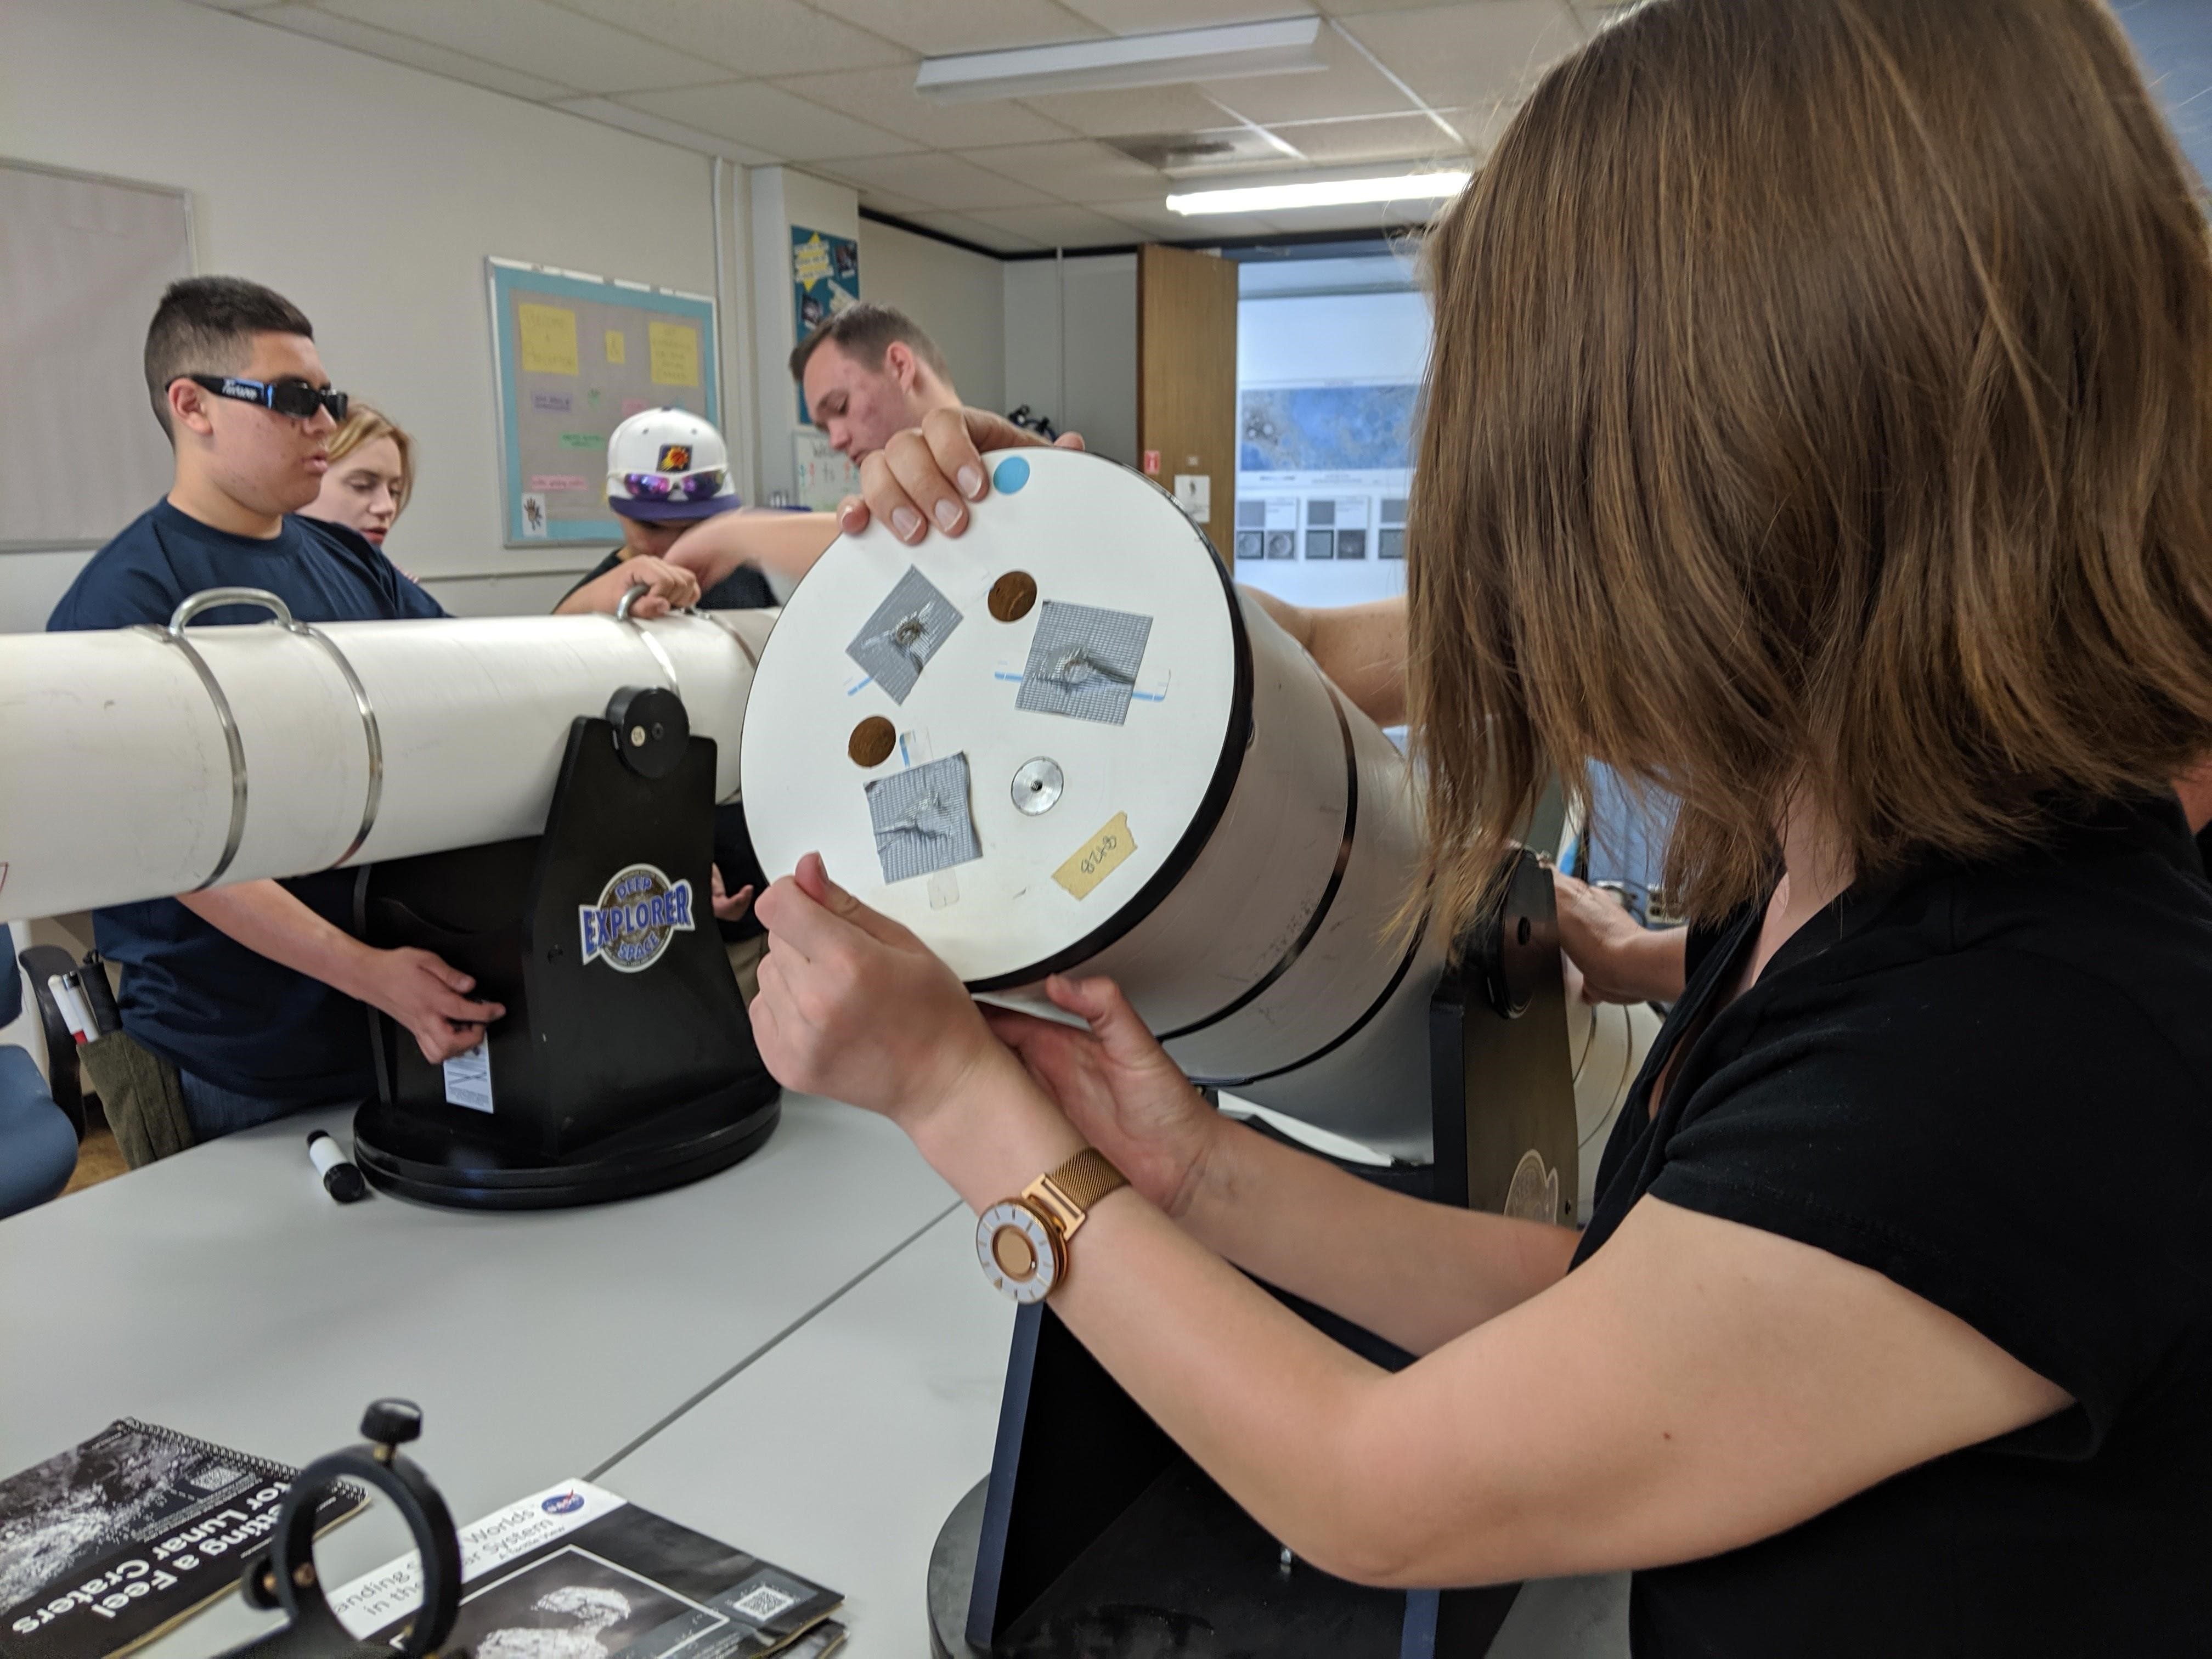
\includegraphics[width=8.5cm]{Project POEM students learn about the parts of a telescope. They are able to take it apart and examine how the telescope is assembled..jpg}
    \caption{Project POEM Enrichment Institute students tactilely explore astronomical telescopes. They were guided to take it apart and put it back together to gain an understanding of how the telescopes are made and how they work. }
    \label{Project POEM students learn about the parts of a telescope. They are able to take it apart and examine how the telescope is assembled.}
\end{figure}
Students stayed in the university dormitory and had an opportunity to simulate college students’ life. Interviews with faculty members, college students with VI, disability resource center staff members, and career counselors were arranged as part of the visit.

Students met in small groups every afternoon based on the Exploration Activities project topic they selected. Each group was co-facilitated by a senior project personnel member and a doctoral student from STEM majors. They worked as a group to prepare a 15–20-minute presentation for the Project POEM Symposium held on the last morning in the College of Astronomy’s telepresence room. This final presentation served as the culminating experience for all participating students in the project and finalized their experiences. 

While Exploration Activities utilized remote le-\\arning from the inception of the project, the Readiness Academy and Enrichment Institute utilized in-person meetings and hands-on experiences as significant means of constructing instructional learning methods. This was especially important for students with VI as tactile learning, hands-on experiences, adaptations for STEM, project design and delivery, and disability-specific skills all require direct instructional modes. The pandemic has impacted how students with VI were taught and how instructional strategies were implemented. Much of the curriculum has been adapted to an online format, and instructional delivery models for our activities had to be updated in 2019. However, the long-term consequences of such adaptations were unknown at the time. It was perceived that the changed format would impact learning pedagogy affecting both students and teachers. After the outbreak of COVID-19 pandemic, we came up with a mitigation practice based on previous study findings (Supalo et al., 2014; Wedler et al., 2014) and recommendations of the project’s advisory committee. For example, 3D printed models, virtual conference tools, online communicational methods (e.g., WhatsApp messenger) were considered for providing realistic and hands-on science and engineering learning as originally intended. 

The decision-making process was conducted based on the collaboration of interdisciplinary team members, including teachers of students with VI, scientists, researchers, mentorship experts, individuals with blindness or low vision working in STEM field and the advisory committee members serving students with VI in school settings. In the following section, we would like to document adaptations implemented during the process and significant takeaways that we had experienced. At the same time, program delivery and instructional strategies were updated in response to the pandemic. In the following section, we would like to document adaptations implemented during the process and significant takeaways that we had experienced. 

\section*{Adaptations to the Readiness Academy}

The Sky School staff had not offered any programming in-person or virtual to anyone in the Tucson community during the pandemic. When Project POEM staff approached Sky School staff to ask if they would assist Project POEM in providing the Readiness Academy virtually, they agreed. 

The Readiness Academy, proposed initially as a five-day on-site experience at the UA’s Sky School located on the summit of Mount Lemmon, was altered in 2021 to be a virtual experience. National Science Foundation granted the POEM staff permission to invite one more cohort of participants to engage in the 14-month intervention beyond the 2020 end date. The pilot phase of the study was conducted from June 2017 to June 2018. There were nine students with VI who completed the pilot study. Of the nine students participating in the Readiness Academy, four students were between grades 6 – 8, and five students were between grades 9 – 12. Four students self-identified as Hispanic, four as White and one as White/American Indian. All students had VI and attended public schools. During the pilot year, both Readiness Academy and Enrichment institute were conducted in person while exploration activity was done remotely.

The nine participating middle and high school students met via Zoom for eight days in the latter part of June. Students had two one-hour Zoom meetings each day where they would either convene as a whole group or in one of the three smaller groups to which they were assigned, based on their specific area of interest. Themes for this group were driven by the Sky School instructors’ areas of knowledge and expertise. By spring 2021, Sky School staff hired dendrochronology (i.e., study of tree rings), wildlife conservation, and atmosphere/climate. Each extension study student participant decided which areas they wanted to learn about and then was assigned to that group. The academy provided adapted learning materials converted from visual-intensive learning materials to accessible tactile graphics and enlarged prints that assist independent activity engagement. The cohort participant experienced the data observation and analysis processes as scientists scientifically conduct in the field. 

Prior to the students attending the virtual Readiness Academy, the Sky School staff created kits that were sent to the students. Each of the virtual daily sessions followed a similar flow, where the first hour was dedicated to getting organized and allowing the students to ask questions. The students practiced new skills during the second hour or applied what they learned from the first hour. For example, if they had received a new tool, such as a talking thermometer, they may have learned how to use that instrument during the first hour and then applied it during the second hour. In addition, they collected data and did activities related to their area of interest and questions they wanted to address during the third and final hour of the session. For example, a student wanted to find out ways that auditory data could be captured using a smartphone. Eventually, this question could lead to the final presentation where the group recorded the environmental sound of busy and quiet communities and made a comparison between the two settings using sound data. 

POEM staff agreed that participants should have some additional equipment and materials to make the adaptations for the Readiness Academy more effective. Science instructors requested a talking thermometer to measure temperature variations on Mt. Lemmon, and a voice recorder to easily keep track of science data. Dr. Kortenkamp successfully worked with a representative of the UA laboratory of tree ring lab research to acquire real samples of tree rings for those participants working in the dendrochronology group. The tree ring samples were tactually accessible to identify age of trees from which samples were taken.

Each of the virtual daily sessions followed a similar flow, where the first hour was dedicated to getting organized and allowing the students to ask questions. The students practiced new skills during the second hour or applied what they learned from the first hour. For example, if they had received a new tool, such as a talking thermometer, they may have learned how to use that instrument during the first hour and then applied it during the second hour. During the third and final hour of the session, they collected data and did activities related to their area of interest and questions they wanted to address.

 Project POEM staff made every effort to emulate the intended processes of the in-person Readiness Academy. The three science instructors were responsible for delivering content and facilitating the small groups of 2–3 students. These science instructors also received in-service training about how to work with students with VI effectively. The instructors participated in four hours of prerequisite training. The training covered topics such as the best instructional methods for working with students with VI, examples of hands-on strategies, common scenarios of science lessons for students with VI, and basic orientation and mobility techniques. We also included further discussions about ways that scientific equipment be used by POEM students through speech.
 
During the small instructional group sessions, the science instructors led the students through the steps of the science and engineering processes at their assigned times. Scheduling included a one-hour break Monday – Wednesday, in the AM between Zoom sessions to allow students independent study time and rest. The Readiness Academy culminated with student-led presentations and was attended by Project POEM staff and parents. In the traditional Sky School experience, there were associates—TVI graduate students, who assisted with activities. For the virtual Readiness Academy, a participant from the Project POEM pilot study was the Sky School Associate. This individual’s role was to provide support with the use of technology. This former participant was very helpful in supporting the POEM participants’ use of technology. She suggested specific keyboard commands used by a screen reader, provided ideas for organizing visual data, and problem-solved together with participants when there were technology-related challenges.

Project POEM staff credited the science instructors with the success of the Readiness Aca-\\demy for the extension study students with VI. Even with last year’s challenges, the instructors were able to “build up some sense of cohesion and unity.” through mini games in virtual settings. At the same time, they let students have fun by playing games with them and doing other relaxing activities. 

At the conclusion of the Readiness Academy, the students gave presentations to each other, Project POEM staff, and their parents. Even though the students could not physically be on Mount Lemmon at the Sky School, they had a positive experience doing the Readiness Academy virtually. 

Perhaps one of the most significant challenges for the Sky School that year was figuring out the accommodations for each student since they would not be on-site. This involved learning what types of devices, programs, and assistive technologies the students were most familiar with and could use to complete the activities. When meeting in-person through the two previous years, staff were dealing with this challenge one-on-one with each student. The student could see a demonstration of a device, technology, or new software program onsite, but the virtual nature of the challenge led to having some of the technology challenges worked out virtually, on a case-by-case basis. For example, one student only had a cell phone so entering data into a tool like an Excel spreadsheet was difficult. The team worked out a solution so that the student would enter the notes into her phone and then verbally relate them to the instructor, who would enter them into the spreadsheet. Even if students were not familiar with a tool, they learned to use it to participate quickly. Guidance was provided by the past POEM participant who was well versed in technology and the POEM experiences. An example of new software that many students learned to use was the Google spreadsheet. 

\section*{Adaptations to the Exploration Activities}
Minor tweaks were made to the Exploration because of the transition to a virtual environment. The team was more intentional about providing guidance to the students and clarifying the assignment and presentation expectations. For example, the students in the pilot study needed to record and submit a presentation after each curriculum segment. The curriculum experienced by the pilot study students comprised six segments, with each segment pushed out approximately every six weeks. The number of segments increased to 10 for the expansion study, so students received a segment approximately once a month but only needed to submit a presentation for eight of the ten segments. The curriculum for the extension study has 11 segments. This change was based on feedback received after the pilot study. A Project POEM staff member reported that the presentations had increased in quality, so they thought these minor changes impacted.

Another adaptation between the pilot and expansion studies was to reduce the number of activities. This was partly due to the transition to a virtual platform, but staff also realized that when students were on-site, they were busy from morning to night. Prior to knowing they had to switch to virtual, Project POEM staff discussed how to incorporate more breaks into the schedule. Project POEM staff learned how to better space out the interactions with the online setting.

Responding to the needs and interests of students also helped improve engagement. To help meet the needs of the students, Project POEM staff first held a virtual meeting with the students two weeks prior to the Enrichment Institute to learn about their interests and explain how the Enrichment Institute was going to work virtually. From this meeting, students were assigned to groups with similar interests. After the meeting, Project POEM staff assembled the necessary materials and mailed them to the students. Students also had access to asynchronous recorded sessions to learn how to use the materials in the box. Then, the groups would meet in a synchronous session to discuss and reflect upon the experiments. Materials include a square board (for one student who is blind to organize her materials), a long wooden stick with a hole carved into the end to launch the projectile, paper plates that serve as mortar holders, safety equipment, e.g., goggles and gloves, three sets of clamps, spray bottles to use to spray water onto craters to enhance drying process, second wooden stick serving as a ruler measure, two dixie cups with a metal nut to tie to a string that is secured to a wooden stick with a hole to measure the projectile distance of impactor, variety of impactors, sizes, shapes, and materials, a Ziploc bag with 10 lbs. of mortar, and scale.

\section*{Adaptations of the Enrichment Institute}

In the past, there were two parts to the weeklong Enrichment Institute. First, students participated in PBL activities. Second, there was a college experience aspect. Because of the pandemic, the Project POEM team had to make some changes to both parts of the Enrichment Institute. For the college experience part, the pilot study students spent a week at the UA campus living in dorms, using food cards, and getting full exposure to campus life. The campus was closed to visitors in Summer 2020, so the expansion study students were unable to participate in this aspect.

To ensure that the expansion study students still had some opportunity to experience college life, a Project POEM staff member worked with universities in Arizona, California, and Colorado to see if there were ways in which the students could learn about the campuses. Project POEM staff created a list of things the universities should cover and worked with individuals on the campuses to ensure these items were included. For example, Project POEM staff members contacted the University of Northern Colorado who agreed to help. A contact at Arizona State University’s Student Accessibility and Inclusive Learning Services said he could help create something for students interested. Because California state schools were closed, all other students were provided an option of participating in a virtual tour at UA. 

The PBL aspect of the Enrichment Institute was held successfully in the virtual environment. The Enrichment Institute consisted of a two-hour planning meeting on May 29 and five days of recorded/asynchronous (a.m. sessions) and remote/live gatherings (p.m. sessions) on June 14–18. When Project POEM staff first met to discuss what they would do for the Enrichment Academy, they started with the question, “How can we make what we did live meaningful for kids in a virtual format?” One of the project staff members had been teaching college students virtually and suggested that his techniques with the college students may also work for the Project POEM students. For example, the staff member created prerecorded asynchronous YouTube videos that the Project POEM students reviewed prior to meeting as a group. These prerecorded messages included instructions on how to unpack the box they received or other instructions related to the upcoming lesson. Staff instructions about how to account for all the box contents and what to do with them were orally communicated in a specific and detailed way. After viewing the recording, the students had approximately an hour to prepare and follow the instructions. Then the students, Project POEM staff, and the university mentors would meet virtually.

Before deciding the content of the lessons, Project POEM staff met with the students to discuss their interests and what they would like to learn related to STEM. Students agreed to learn about impact craters from this discussion, so a lesson on impact craters was created. The students received sand and special glue to keep the sand together. Then, the students and Project POEM staff talked about how to drop objects and other research questions they wished to address, such as if size, velocity, or angle mattered. A Project POEM staff member added that they heard the students use the “I wonder” phrase as they asked questions like “little scientists.” The staff member also commented that the student presentation had “gone up a notch” from the pilot study. In fact, for the expansion study, students described what was on the slides, like an instructor would, which was something the students had not done previously. The 3D models for the craters also were successful. These models were created by a Project POEM staff member using NASA programming and programming created by the staff member. Currently, the models are on display with braille labels in the UA’s College of Science.

A success noted in the progression from pilot study to expansion study was retention and level of engagement. As previously mentioned, students were asked to submit presentations for eight of the ten segments in the expansion study. More than 80 percent of the students submitted the presentations, which exceeded the expectations of the Project POEM staff members. 

When asked why students in the expansion study seemed to be more engaged, a Project POEM staff member conjectured that it may have been because of the novelty that a student with VI could do hands-on science experiments. Another potential reason may be that, when students were recruited, they were told it was a science-based extracurricular type program. Some of the engagement may be due to the new communication measures Project POEM implemented (i.e., switching from “Desire2Learn” learning management platform during the pilot study), to text message groups during the first year, and finally to WhatsApp Messenger during the second pandemic year), or the students may have been more interested in science compared to the students in the pilot study, a staff member said. 

According to a staff member, another adaptation made between the pilot study and expansion study was a reduction in the number of activities. This was partly due to the transition to a virtual platform, but staff also realized that when students were on-site, they were busy from morning to night. Prior to knowing they had to switch to virtual, Project POEM staff discussed how to incorporate more breaks into the schedule. Project POEM staff learned how to better space out the interactions for the online setting.

Responding to the needs and interests of students also helped improve engagement. To help meet the needs of the students, Project POEM staff first held a virtual meeting with the students two weeks prior to the Enrichment Institute to learn about their interests and explain how the Enrichment Institute was going to work virtually. From this meeting, students were assigned to groups with similar interests. After the meeting, Project POEM staff assembled the necessary materials and mailed them to the students. Students also had access to asynchronous recorded sessions to learn how to use the materials in the box. Then, the groups would meet in a synchronous session to discuss and reflect upon the experiments.

\section*{Implications}

Project POEM successfully adapted to the intervention project's Readiness, Exploration, and Enrichment phases targeted for students with VI. Overall, the pandemic and its impacts on instruction put educators in situations where they must imagine and deliver high-level education to students where some of the learning activities are virtually delivered. Due to the changes from hands-on to virtual environments, some were implemented from previous years' feedback to increase engagement and retention. 

Throughout the one-year practice after the pandemic, the researchers evaluated a total of 64 STEM presentations recorded by the student participants. According to Kortenkamp et al. (2022), the adaptations positively impacted the project components on the project’s intended outcomes: 1) Communication and organization in STEM, 2) Energy and confidence in communicating ideas and information, and 3) Presenting presentation prompts. Also, we found that the adaptations succeeded in student participants’ retention and assignment submission rates (84\%, 64 of 80 presentation assignments submitted).

To address this transition, a team of educators from diverse backgrounds collaborated to adapt curricula and reached successful outcomes. Project POEM is an example of one of those curricula/outcomes for students with VI. This project’s emphasis on a team-based approach was paramount to a successful outcome for students with VI learning a content area in a virtual environment. Teams with experts knowledgeable in several areas (e.g., STEM area, VI learning differences, accessible and assistive technology) covered all the knowledge and skill differences that the participants may bring to the learning situation. The realization that a virtual STEM curriculum was attainable with several implications as the original components were transformed to engage students with VI in online learning.

First, technology plays a significant role in implementing and operating students learning experiences. An important discovery was that not all participants were knowledgeable in utilizing technology for online learning before the pandemic, such as web-based applications (e.g., Google spreadsheets) and conferencing platforms (e.g., Zoom). Our adaptations provided opportunities for students to learn new technology and platforms to facilitate participation in POEM activities. 

Second, careful guidance and specific instruction to allow independent and self-initiated participation of students made it possible for the program to combine various types of activities remotely. Participant students benefited from their STEM courses and other areas in learning and independence. Programs that offer STEM activities can be open to participants with VI learning new technologies/software. Project POEM adaptations led to a greater understanding of STEM activities delivered in-person and through online learning. Combining these two instructional delivery systems led to more variety of learning opportunities and preserved hands-on learning, which is important not only to students with VI, but all students engaged in STEM activities. With video sharing services (e.g., YouTube), participants could access videos for experiment demonstrations, assembling a model, and general explanations. The services also allowed POEM participants to record their STEM activities to share with others and critique their experiences. This adaptation allowed science programs to be delivered asynchronously for all students’ success in online learning. Inclusive design of virtual online learning can work for all students if carefully planned and designed through the expertise of people with diverse backgrounds to engage in STEM activities.

Third, planning in advance played a critical role and collaborative participation of all team members was essential. POEM staff and other scientists working with POEM met regularly through email and primarily through zoom meetings. When the Sky School Readiness Academy went through major adaptations, Ms. Lipson, Sky School director, met numerous times with POEM staff and her dedicated scientists to restructure the academy, including live zoom meetings and participant independent study. Dr. Kortenkamp, who is a POEM scientist, also met with POEM staff to restructure the Enrichment Academy, which resulted in a multi-faceted delivery of material and interaction with participants, e.g., YouTube videos to view and then real-time meetings with Dr. Kortenkamp, independent study at participants’ homes to complete experiments and then coming together as a group to give presentations. Communication was improved after the POEM pilot study by implementing the WhatsApp Messenger system, which was an easy way for mentors and mentees to exchange ideas one on one or in small groups. Project POEM staff noticed that communication was faster and more flexible when the app was implemented beginning the second project year.

POEM’s hands-on materials mailed to participants’ homes were available to provide realistic STEM experiences in in-person and virtual settings. During the pandemic, the participants worked remotely using 3D printing models and 2D tactile graphics. The availability of these materials increased the possibility of the participants understanding STEM concepts and raising questions about the solar system. Accessible communication platforms (e.g., WhatsApp Messenger) helped smoothen the transition from hands-on to virtual learning environments.

\section*{Conclusion}

Program adaptations for Project POEM during the Covid-19 pandemic were beneficial for students with VI. Using an inclusive learning model, the adaptations implemented can benefit students with VI and those students without disabilities. The adaptations of the program afford many examples of exemplary science learning guided by the NGSS as POEM follows. We identified that the adapted virtual science learning program successfully maintained the participants’ engagement and enthusiasm in STEM areas during the pandemic. We identified that the adapted virtual science learning program successfully maintained the participants’ engagement and enthusiasm in STEM areas during the pandemic. We hope that other educators engaged in STEM can use the adapted POEM activities as a model to develop hands-on activities for all students interested in STEM.

\section*{Acknowledgment}

This study was supported by a grant from the National Science Foundation’s ITEST program (award #1657201) and performed at the University of Arizona. Lodging, meals, transportation, and equipment during the project were all provided free of charge to participants. Any opinions, findings, conclusions, or recommendations are those of the authors and do not necessarily reflect the position or endorsement of the funding agency. POEM is approved for human subject research at the University of Arizona by our Institutional Review Board (IRB #1702248263). In compliance with this approval process, we obtained assent forms from students as well as consent forms from their parents and mentors.


\include{} 
\section*{References}\par 

\leftskip 0.25in
\parindent -0.25in 
%%%

Balster, N., Pfund, C., Rediske, R., \& Branchaw, J. (2010). Entering research: a course that creates community and structure for beginning undergraduate researchers in the STEM disciplines. CBE—Life Sciences Education, 9(2), 108-118.

Foster, E. A., Lepore-Stevens, M., Adams, D., \& Lepore, M. (2020). The Sports Camp Experience Continued During COVID Pandemic for Children with Visual Impairments. PALAESTRA, 34(3), 8-10. 

Handelsman, J., Pfund, C., Lauffer, S. M., \& Pribbenow, C. M. (2005). Entering mentoring. Madison: The Wisconsin Program for Scientific Teaching.

Hamid, S. M. (2020). Online digital platforms during covid-19 in EFL classes: Visual impairment student’ perception. ETERNAL (English, Teaching, Learning, and Research Journal), 6(2), 328-339. 

Kortenkamp S. J., Park J., Alshuli T., Tsinajinie G., Buxner S., Topor I., and Hong S. (2022). Touching the Solar System: A Project-Based Learning Astronomy Program for Students with Visual Impairments. Connected Science Learning, 4(4).

Lepore-Stevens, M., Adams, D., Lepore, M., \& Foster, E. A. (2021). Camp Abilities: Accessibility and Virtual Summer Camps. Journal of Park \& Recreation Administration, 39(4), 141-151. 

Lunsford, L., Hong, S., Tsinajinie, G., Buxner, S., Topor, I., (in press). Online Mentor Education for Mentors of Youth with Visual Impairments. Journal of Visual Impairments and Research Innovation.

McBride, C. R. (2020). Critical Issues in Education for Students with Visual Impairments: Access to Mathematics and the Impact of the Covid-19 Pandemic [Ph.D., University of Georgia]. Athens GA. 

Mulliken, A. (2017). “There is Nothing Inherently Mysterious about Assistive Technology” A Qualitative Study about Blind User Experiences in US Academic Libraries. Reference and User Services Quarterly, 57(2), 115-126. 

NGSS Lead States. (2013). Next generation science standards: For states, by states. The National Academies Press. https://doi.org/\\10.17226/18290

Rosenblum, L. P., Herzberg, T. S., Wild, T., Botsford, K. D., Fast, D., Kaiser, J. T., Cook, L. K., Hicks, M. A. C., DeGrant, J. N., \& McBride, C. R. (2020). Access and Engagement: Examining the Impact of COVID-19 on Students Birth-21 with Visual Impairments, Their Families, and Professionals in the United States and Canada. https://static.afb.org/legacy/media/AFB\_\\Access\_Engagement\_Report\_Accessible\_FI\\NAL.pdf

Smith, C. (2020). Challenges and opportunities for teaching students with disabilities during the COVID-19 pandemic. International Journal of Multidisciplinary Perspectives in Higher Education, 5(1), 167-173.

Supalo, C. A., Isaacson, M. D., \& Lombardi, M. V. (2014). Making hands-on science learning accessible for students who are blind or have low vision. Journal of Chemical Education, 91(2), 195-199.

Tal, T., Krajcik, J. S., \& Blumenfeld, P. C. (2006). Urban schools' teachers enacting project‐based science. Journal of Research in Science teaching, 43(7), 722-745. 

Wedler, H. B., Boyes, L., Davis, R. L., Flynn, D., Franz, A., Hamann, C. S., ... \& Wang, S. C. (2014). Nobody can see atoms: Science camps highlighting approaches for making chemistry accessible to blind and visually impaired students. Journal of Chemical Education, 91(2), 188-194.




\include{} 


\endleftskipleftskip 
\endparindentparindentparindentparindent

\end{large}
\end{document}
